\chapter{Arhitektura i dizajn sustava}
		
		Arhitekturu našeg sustava možemo podijeliti na tri podsustava:	
		\begin{itemize}
		\item 	\textit{Web preglednik}
		\item 	\textit{Baza podataka}
		\item 	\textit{Web poslužitelj}		
		\end{itemize}
		
		\begin{figure}[H]
			\centering
			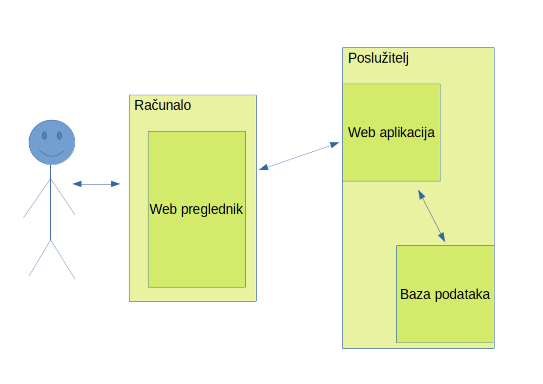
\includegraphics[width=\textwidth, scale=2.0]{slike/arhitektura.png}
			\caption{Arhitektura našeg sustava}
			\label{fig:arhitektura}
		\end{figure}
\eject
	
	\underbar{ \textit{Web poslužitelj}}{ je srce našeg sustava. Njegova zadaća je komunikacija klijenta s aplikacijom te bazom podataka. Pri komunikaciji koristi HTTP protokol. Poslužitelj služi za prosljeđivanje zahtjeva koji se naknadno obrađuju.}
	
	\underbar{ \textit{Web preglednik} }{je program koji korisniku omogućuje pregled web-stranica i multi-medijalnih sadržaja vezanih uz njih. Korisnik putem web preglednika šalje zahtjeve na obradu poslužitelju.}
	
	\underbar{ \textit{Baza podataka}}{ je zbirka zapisa pohranjenih u računalu na sustavan način, tako da joj se računalni program može obratiti prilikom odgovaranja na problem. Web poslužitelj komunicira s bazom podataka te povlači potrebne zapise iz nje.}
	{Klijent koristi web aplikaciju za slanje određenih zahtjeva. Zahtjev se obrađuje, te se kao odgovor na zahtjev prikazuje HTML dokument.}
	\\
	{Pri izradi web aplikacije koristili smo Java Spring Boot iz Spring framework-a zajedno sa Reactom na klijentskoj strani. Korišteno je razvojno okruženje IntellJ IDEA.}
	{Arhitektura sustava temeljiti će se na MVC (Model-View-Controller) konceptu. Prednosti korištenja MVC arhitekture je taj što je moguće nezavisno razvijanje i spajanje u cjelinu što uvelike olakšava razvoj aplikacije.}
	
	 {Model-View-Controller se sastoji od:}
	\begin{itemize}
		\item 	\textbf{Model} {je centralni dio aplikacije, koja obuhvaća promjenljivu (dinamičku) strukturu podataka, direktno upravljanje podacima, logikom i pravilima aplikacije}
		\item 	\textbf{View}{ je bilo koji izlazni prikaz podataka u korisničkom okruženju, pri čemu se isti podaci mogu prikazati na više načina}
		\item 	\textbf{Controller} {ulazne podatke pretvara u komande koje upravljaju modelom ili prikazom podataka u korisničkom okruženju}
	\end{itemize}
	
		\begin{figure}[H]
			\centering
			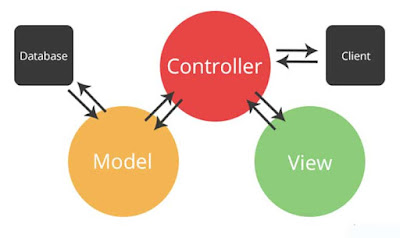
\includegraphics[width=100mm, scale=0.1]{slike/MVC.jpeg}
			\caption{MVC model}
			\label{fig:arhitektura}
		\end{figure}
\eject

		

				
		\section{Baza podataka}
			
			
			
		Za potrebe naseg sustava koristit cemo relacijsku bazu podataka koja svojom strukturom olaksava modeliranje stvarnog svijeta. Gradivna jedinka baze je relacija, odnosno tablica koja je definirana svojim imenom i skupom atributa. Zadaca baze podataka je brza i jednostavna pohrana, izmjena i dohvat podataka za daljnju obradu.
Baza podataka ove aplikacije sastoji se od sljedecih entiteta: 
\begin{itemize}
		\item korisnikAplikacije
		\item uloge
		\item pokusajDoniranja
		\item krvnaVrsta
		\item potrosnjaKrvi
		\item aktivacijskiKodovi
		\item adresa
		
	\end{itemize}

		
			\subsection{Opis tablica}
			

				\textbf{korisnikAplikacije \textit{•}}
				 Ovaj entitet predstavlja sve korisnike apliakacije (admin,djelatnik,donor) i diferencira ih pomoću ulogaId što je referenca na tablicu uloga. KorisnikId i lozinka se koristi za login u aplikaciju, ako korisnik još nije aktivirao svoj račun, onda u atributu lozinka stoji null. Za admina i djelatnika postoje atributi : ime, prezime, oib dok su ostale vrijednosti null. Kod stvaranja atributa trajnoOdbijanjeDarivanja je false, a razlogOdbijanja je null ,ako se korisniku odbije darivanje zauvijek onda se ti atributi mjenjaju.
				
				
				\begin{longtblr}[
					label=none,
					entry=none
					]{
						width = \textwidth,
						colspec={|X[15,l]|X[6, l]|X[20, l]|}, 
						rowhead = 1,
					} %definicija širine tablice, širine stupaca, poravnanje i broja redaka naslova tablice
					\hline \multicolumn{3}{|c|}{\textbf{korisnikAplikacije}}	 \\ \hline[3pt]
					\SetCell{LightGreen}korisnikId & VARCHAR & id pomocu kojeg se korisnik prijavljuje u sustav (jednako donorid za donore) -> Generira se pomoću inicijala i zadnjih 5 znamenki oiba npr.
					Ivica ivic 0303041001340 ima korisnikId = ii01340\\ \hline
					lozinka	& VARCHAR &  lozinka za login (nullable)	\\ \hline 
					ime & VARCHAR	&  ime korisnika		\\ \hline 
					prezime & VARCHAR	& prezime korisnika	\\ \hline 
					mjestoRodenja & VARCHAR & mjesto na kojem se korisnik rodio (nullable) \\ \hline
					oib & NUMERIC(11) & oib korisnika \\ \hline
					\SetCell{LightBlue} adresaStanovanja & INT & id adrese na kojoj korisnik stanuje ( instancirana u tablici adrese vezom 1 naprema *) (nullable) \\ \hline
					mjestoZaposlenja & VARCHAR & firma u kojoj je korisnik zaposlen (nullable) \\ \hline
					email & VARCHAR & email na koji korisniku dolaze korisne informacije (nullable) \\ \hline 
					brojMobitelaPrivatni & INT	&  broj na koji korisniku dolaze korisne infromacije privatni	(nullable)	\\ \hline
					brojMobitelaPoslovni & INT	&  broj na koji korisniku dolaze korisne infromacije poslovni ( ne obavezan za sve uloge) (nullable)		\\ \hline
                     datumRodenja & DATE &  datum rodenja (nullable)	\\ \hline
                     trajnoOdbijanjeDarivanja & Boolean	&  (nullable)		\\ \hline
                     razlogOdbijanja & VARCHAR	&  	kratki opis razloga odbijanja	\\ \hline
					\SetCell{LightBlue} uloga id	& INT &  označuje da li je korisnik admin, djelatnik ili donor 	\\ \hline 
				\end{longtblr}
				
				\textbf{uloge \textit{•}}
				entitet koji sadrži dva atributa, id za oznaku rednog broja uloge i ulogaName za ime 						uloge
				\begin{longtblr}[
					label=none,
					entry=none
					]{
						width = \textwidth,
						colspec={|X[6,l]|X[6, l]|X[20, l]|}, 
						rowhead = 1,
					} %definicija širine tablice, širine stupaca, poravnanje i broja redaka naslova tablice
					\hline \multicolumn{3}{|c|}{\textbf{Uloge}}	 \\ \hline[3pt]
					\SetCell{LightGreen}ulogaId & INT	& označuje id uloge (admin, djelatnik ili donor)\\ \hline
					ulogaName	& VARCHAR & ime uloge(donor,admin...)  	\\ \hline 
				\end{longtblr}
				\textbf{pokusajDoniranja\textit{•}}
				-entitet koji služi za spremanje pokusaja doniranja, sprema podatke o datumu, mjestu, darivatelju, djelatniku, uspješnosti i razlogu odbijanja ako je uspješnost negativna
				
				\begin{longtblr}[
					label=none,
					entry=none
					]{
						width = \textwidth,
						colspec={|X[15,l]|X[6, l]|X[20, l]|}, 
						rowhead = 1,
					} %definicija širine tablice, širine stupaca, poravnanje i broja redaka naslova tablice
					\hline \multicolumn{3}{|c|}{\textbf{pokusajDonacije}}	 \\ \hline[3pt]
					\SetCell{LightGreen}brDoniranja & VARCHAR & redni broj donacije\\ \hline
					datum & DATE & datum donacije \\ \hline
					mjestoDarivanja	& VARCHAR & opisno mjesto donacije	\\ \hline 
					\SetCell{LightBlue}korisnikIdDjelatnika & VARCHAR & korisnikId od djelatnika \\ \hline
					\SetCell{LightBlue}korisnikId & VARCHAR & korisnikId od donora \\ \hline

					uspjeh	& boolean & true za uspjeh, false za neuspjeh  	\\ \hline 
					razlogOdbijanja & VARCHAR & opis zašto je korisnik odbijen \\ \hline
					
					
					
				\end{longtblr}
				
				\textbf{krvnaVrsta\textit{•}}
				
				- entitet čuva podatke o zalihi i predviđenim zalihama svih krvnih grupa
				\begin{longtblr}[
					label=none,
					entry=none
					]{
						width = \textwidth,
						colspec={|X[15,l]|X[6, l]|X[20, l]|}, 
						rowhead = 1,
					} %definicija širine tablice, širine stupaca, poravnanje i broja redaka naslova tablice
					\hline \multicolumn{3}{|c|}{\textbf{krvnaVrsta}}	 \\ \hline[3pt]
					\SetCell{LightGreen}krvId & SERIAL & ID krvi serial \\ \hline
					imeKrvneGrupe & VARCHAR & (A+,A-,AB+,B-...) \\ \hline
					gornja granica & INT & gornja granica dopuštene količine krvi u jedinicama\\ \hline

					donja granica	& INT & donja granica dopuštene količine krvi u jedinicama  	\\ \hline 
					trenutna zaliha	& INT &  trenutna zaliha konkretne krve grupe u jedinicama 	\\ \hline 
					
					
				\end{longtblr}
				
				
				\textbf{potrosnjaKrvi\textit{•}}
				
				entitet koji prati isporuke krvi
				\begin{longtblr}[
					label=none,
					entry=none
					]{
						width = \textwidth,
						colspec={|X[15,l]|X[6, l]|X[20, l]|}, 
						rowhead = 1,
					} %definicija širine tablice, širine stupaca, poravnanje i broja redaka naslova tablice
					\hline \multicolumn{3}{|c|}{\textbf{potrosnjaKrvi}}	 \\ \hline[3pt]
					\SetCell{LightGreen} idPotrosnje & SERIAL & Redni broj isporuke krvi \\ \hline
					timestampPotrosnje & timestamp & timestamp potrošnje \\ \hline
					\SetCell{LightBlue}krvId & INT & id krvne grupe \\ \hline
					količinaJedinica 	& INT &  broj jedinica koji su se potrošili 	\\ \hline 
					
					\SetCell{LightBlue} korisnikIdDjelatnika & VARCHAR &  korisničko ime djelatnika koji je inicirao slanje krvi bolnici	\\ \hline 
					lokacijaPotrosnje & VARCHAR & opisna lokacija kamo ide isporuka krvi \\ \hline
					
				\end{longtblr}
				
				\textbf{adresa\textit{•}}
				
				entitet koji sprema sve adrese korisnika sustava
				\begin{longtblr}[
					label=none,
					entry=none
					]{
						width = \textwidth,
						colspec={|X[10,l]|X[6, l]|X[20, l]|}, 
						rowhead = 1,
					} %definicija širine tablice, širine stupaca, poravnanje i broja redaka naslova tablice
					\hline \multicolumn{3}{|c|}{\textbf{adrese}}	 \\ \hline[3pt]
					\SetCell{LightGreen}idAdrese & SERIAL & id adrese \\ \hline
					postanskiBroj & INT & poštanski broj adrese \\ \hline
					mjesto 	& VARCHAR &  mjesto u adresi 	\\ \hline 
					ulica & VARCHAR & ulica adrese \\ \hline
					brojKuce & VARCHAR & redni broj kuće, može biti i 7a ili 7b pa je zato varchar \\ \hline
					kat & INT & kat na kojem se stanuje, može biti null \\ \hline
					
				\end{longtblr}
				
				\textbf{aktivacijskiKodovi\textit{•}}
				
				entitet koji služi kao spremiše aktivacijskih kodova koji čekaju korisnika da ih potvrdi
				\begin{longtblr}[
					label=none,
					entry=none
					]{
						width = \textwidth,
						colspec={|X[10,l]|X[6, l]|X[20, l]|}, 
						rowhead = 1,
					} %definicija širine tablice, širine stupaca, poravnanje i broja redaka naslova tablice
					\hline \multicolumn{3}{|c|}{\textbf{aktivacijskiKodovi}}	 \\ \hline[3pt]
					\SetCell{LightGreen}korisnikId & VARCHAR & id adrese \\ \hline
					aktivacijskiKljuc & VARCHAR(10) &  ključ koji se generira s kojim korisnik treba potvrditi račun \\ \hline
					
				\end{longtblr}
			
			\subsection{Dijagram baze podataka}
				\begin{figure}[H]
	\centering
	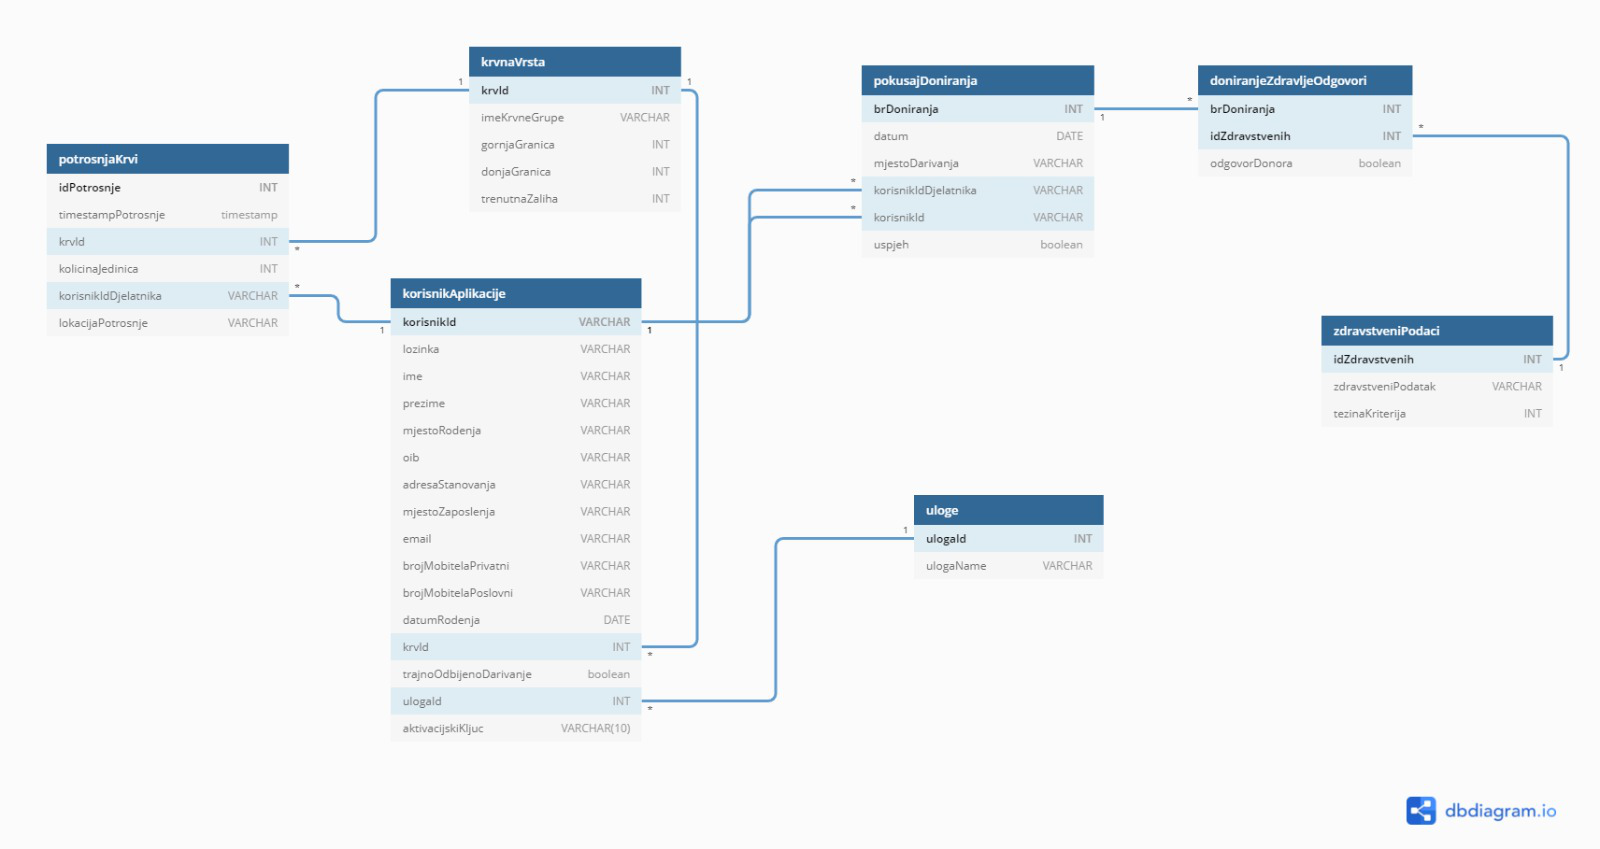
\includegraphics[width=\textwidth, scale=2.0]{dijagrami/relShema.png}
	\caption{relacijski model baze podataka UC8}
	\label{fig:dijagram_baze}
\end{figure}
			\eject
			
		\section{Dijagram razreda}
		
			\textit{Potrebno je priložiti dijagram razreda s pripadajućim opisom. Zbog preglednosti je moguće dijagram razlomiti na više njih, ali moraju biti grupirani prema sličnim razinama apstrakcije i srodnim funkcionalnostima.}\\
			
			\textbf{\textit{dio 1. revizije}}\\
			
			\textit{Prilikom prve predaje projekta, potrebno je priložiti potpuno razrađen dijagram razreda vezan uz \textbf{generičku funkcionalnost} sustava. Ostale funkcionalnosti trebaju biti idejno razrađene u dijagramu sa sljedećim komponentama: nazivi razreda, nazivi metoda i vrste pristupa metodama (npr. javni, zaštićeni), nazivi atributa razreda, veze i odnosi između razreda.}\\
			
			\textbf{\textit{dio 2. revizije}}\\			
			
			\textit{Prilikom druge predaje projekta dijagram razreda i opisi moraju odgovarati stvarnom stanju implementacije}
			
			
			
			\eject
		
		\section{Dijagram stanja}
			
			
			\textbf{\textit{dio 2. revizije}}\\
			
			\textit{Potrebno je priložiti dijagram stanja i opisati ga. Dovoljan je jedan dijagram stanja koji prikazuje \textbf{značajan dio funkcionalnosti} sustava. Na primjer, stanja korisničkog sučelja i tijek korištenja neke ključne funkcionalnosti jesu značajan dio sustava, a registracija i prijava nisu. }
			
			
			\eject 
		
		\section{Dijagram aktivnosti}
			
			\textbf{\textit{dio 2. revizije}}\\
			
			 \textit{Potrebno je priložiti dijagram aktivnosti s pripadajućim opisom. Dijagram aktivnosti treba prikazivati značajan dio sustava.}
			
			\eject
		\section{Dijagram komponenti}
		
			\textbf{\textit{dio 2. revizije}}\\
		
			 \textit{Potrebno je priložiti dijagram komponenti s pripadajućim opisom. Dijagram komponenti treba prikazivati strukturu cijele aplikacije.}
